\section{Analisi dei dati e classificatori utilizzati}

In questa sezione verrà riportato lo studio effettuato sul dataset.
% Ogni sottosezione tratterà di uno specifico classificatore, dei suoi risultati e degli esperimenti fatti per migliorarne il modello.

\subsection{Considerazioni sugli attributi}

Studiando la composizione dei dati per selezionare le principali tecniche da applicare,
la prima cosa che risulta visibile all'apertura del dataset è sicuramente il suo sbilanciamento nelle classi di output:
come mostrato in~\Cref{fig:classes}, su 100 pazienti in esame, solo 12 risultano compromessi.

\begin{figure}[H]
  \centering
  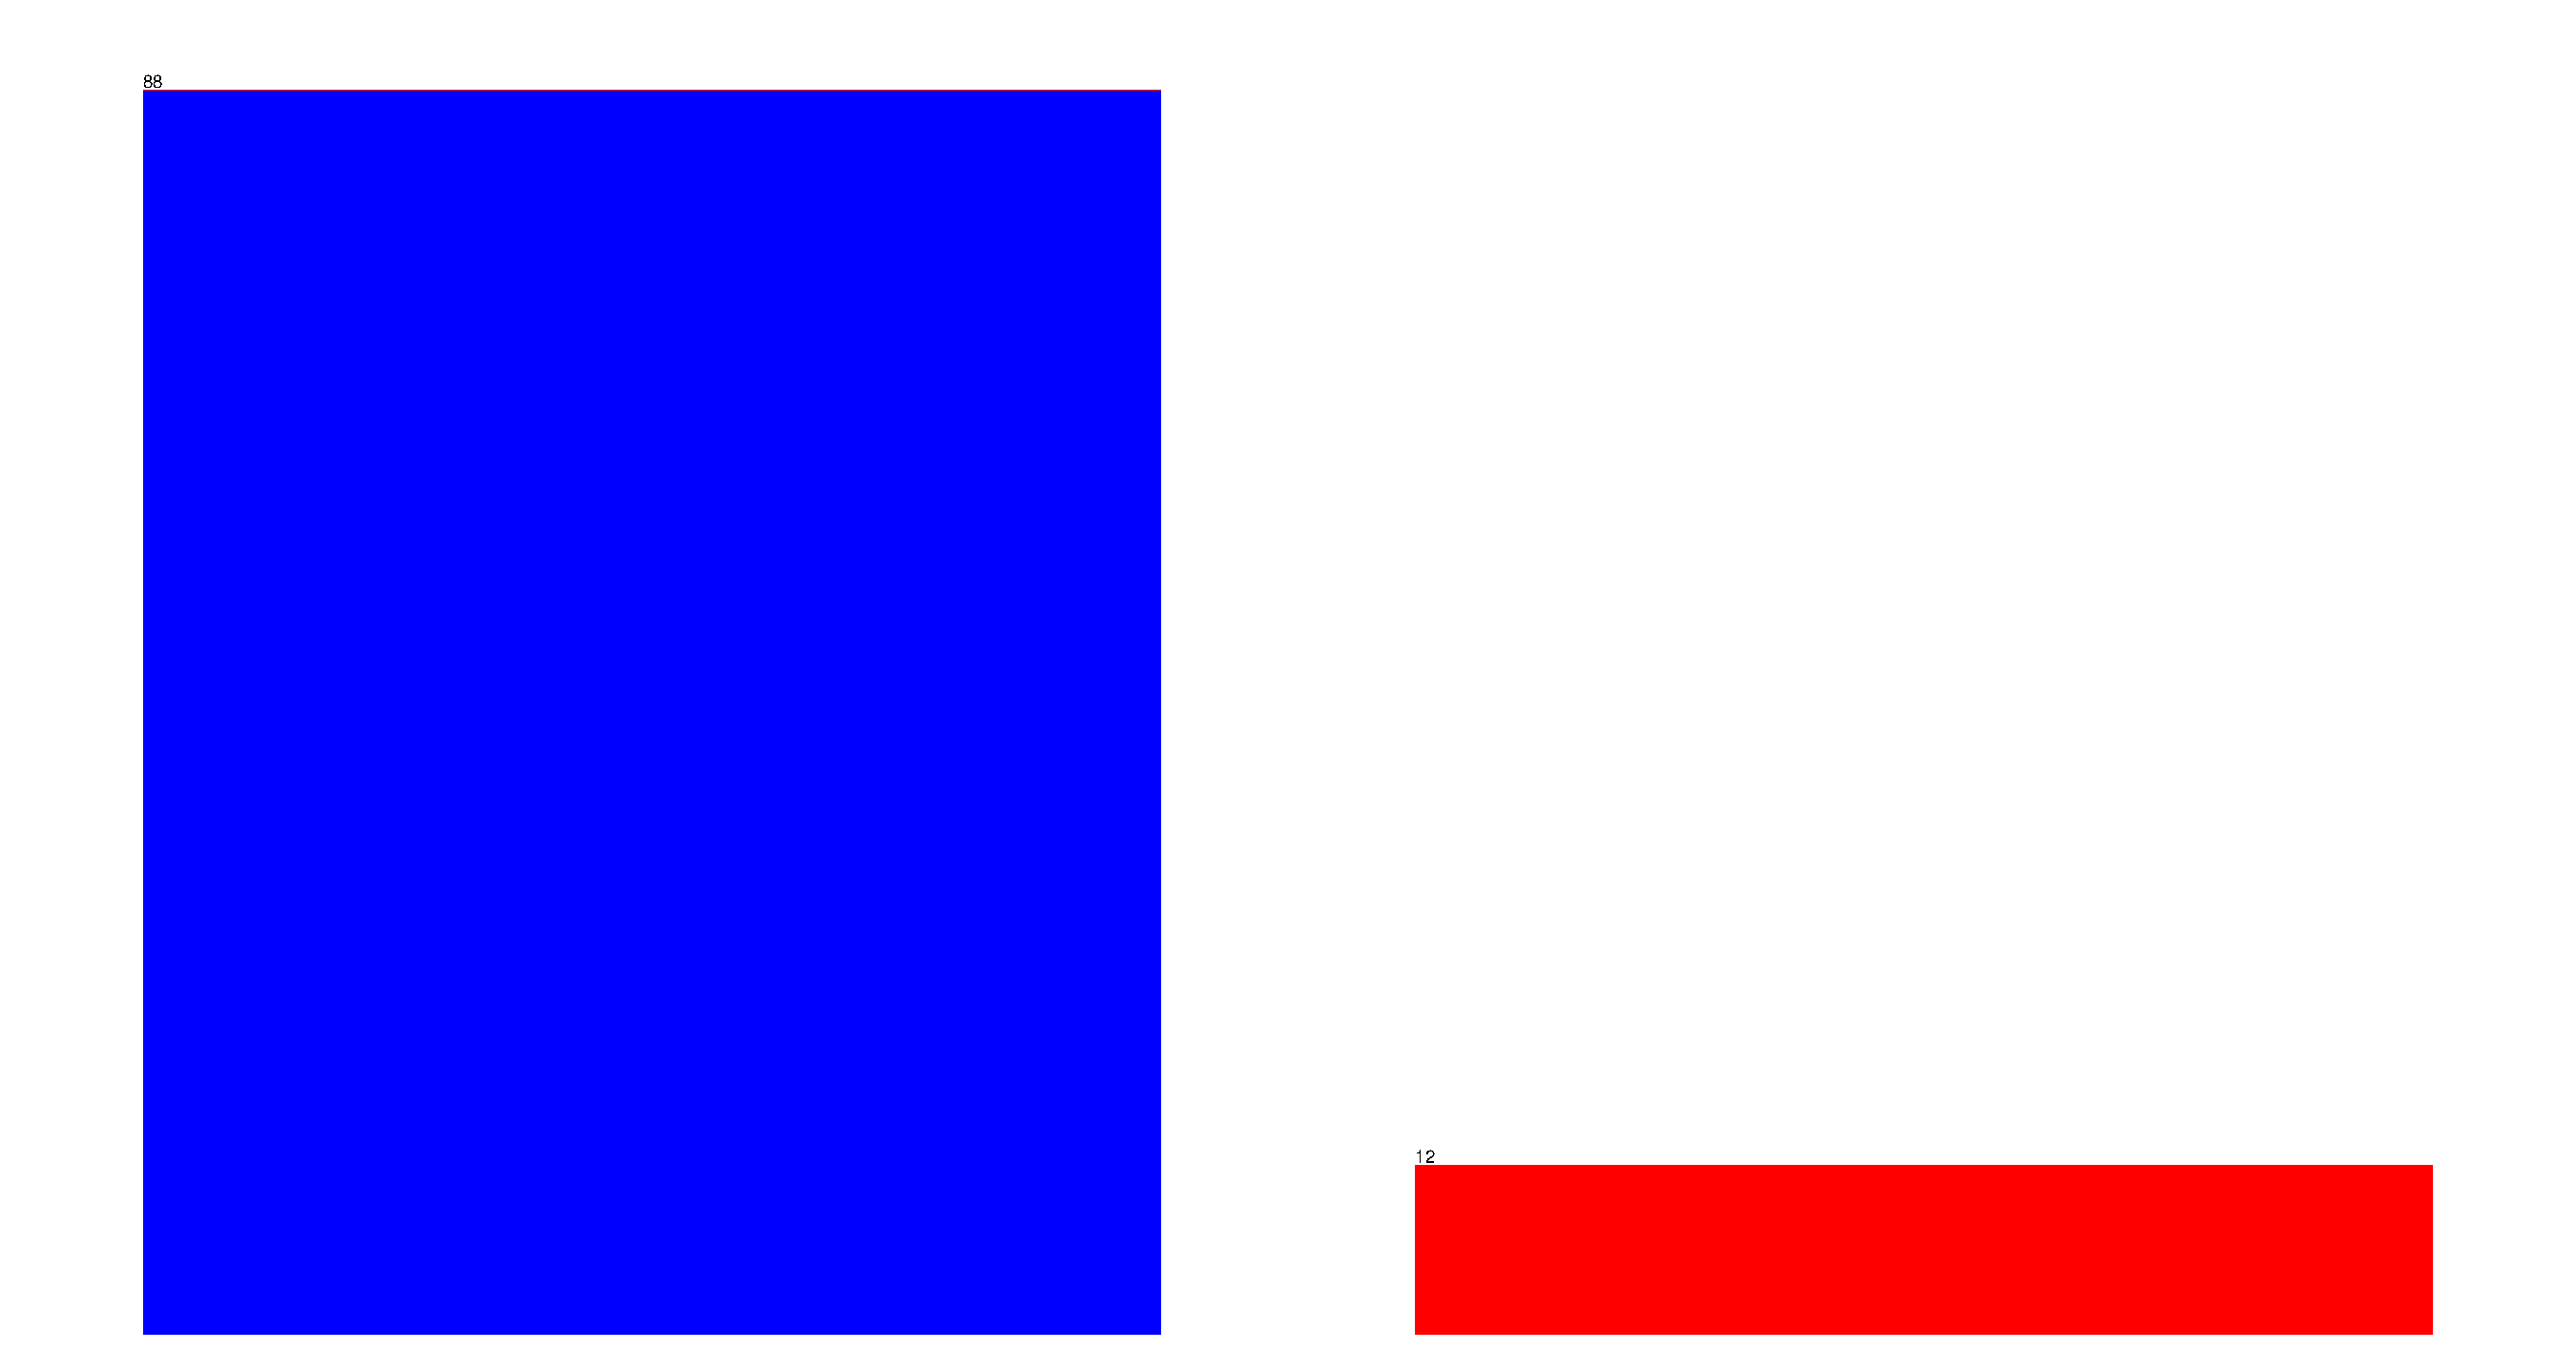
\includegraphics[width=0.85\textwidth]{fig/classes.eps}%
  \caption{%
    L'istogramma rappresenta i valori assunti dall'attributo classe:
    la colonna blu rappresenta le diagnosi di fertilità normale,
    quella rossa gli esami che evidenziano potenziali problematiche.
  }%
  \label{fig:classes}
\end{figure}

Questo disequilibrio tra le classi mette in difficoltà i modelli più semplici;
al fine di ottenere risultati validi, si è messo alla prova diverse configurazioni parametriche.

\todo[inline]{Aggiungere maggiori dettagli per ciascun attributo}

\subsection{Misure di performance dei classificatori}

\todo[inline]{Migliorare quanto segue}

Prima di partire con i vari dati, occorre però stabilire i criteri di misura delle performance dei vari classificatori:
a tale scopo ho tenuto conto in primo luogo della Confusion Matrix prodotta da ogni modello, successivamente dei valori di Precision e Recall per le classi in gioco, attribuendo un maggiore peso ai valori relativi alla classe ``O'' rispetto a ``N'' e infine del valore della ROC\@.
Come modalità di test ho scelto di applicare in ogni situazione la K-Fold Cross-Validation piuttosto che lo splitting statico dei dati in Training e Test Set, la motivazione dietro a questa scelta è l'esiguo numero di dati presenti nel dataset a cui si presta meglio una modalità come il K-Fold Cross-Validation,
in quanto pensata appositamente per dataset di piccole dimensioni.

\todo[inline]{Manca qualcosa?}

\subsection{kNN}
\subsection{Decision Tree}

La prima tecnica di classificazione testata è stata il Decision Tree.
In particolare, si è scelto di usare \texttt{J48}, implementazione dell'algoritmo \emph{C4.5};
esso realizza un albero binario a cui possono essere applicate tecniche di \emph{post pruning}
per ridurre le dimensioni dell'albero e l'errore commesso dal classificatore.

In primo luogo si è provato a generare un modello applicando i parametri standard impostati da Weka, ottenendo così i risultati riportati in~\Cref{fig:j48}.

\begin{figure}[H]
  \centering
  \adjincludegraphics[width=\linewidth,trim=0 0 0 {.3\height},clip]{fig/j48.eps}%
  \caption{Output di J48 eseguito tramite Weka}%
  \label{fig:j48}
\end{figure}

Com'è possibile notare, il classificatore costruisce un modello poco valido:
per quanto \emph{accuracy}, \emph{precision} e \emph{recall} per la classe ``\texttt{N}'' abbiano valori piuttosto elevati,
i corrispondenti per ``\texttt{O}'' risultano tendenti a \(0\).
Anche il valore di \emph{ROC}, indicatore principale della bontà di un modello di classificazione, risulta estremamente basso.

Osservando la struttura dell'albero costruito, è piuttosto chiaro il motivo di valori tanto bassi:
l'albero infatti è costruito da un'unica foglia i cui valori sono assegnati alla classe ``\texttt{N}'', causando così la situazione sopra descritta.

Ovviamente questo modello non risultava di una qualità soddisfacente, probabilmente a causa del post pruning,
il quale, in presenza di un tale sbilanciamento nella frequenza delle classi, tende a ridurre l'albero di classificazione a singola foglia.
Per porre rimedio a questa cosa si è provato ad aumentare e diminuire il parametro \texttt{confidenceFactor}, responsabile di accentuare o smussare le operazioni di pruning;
anche però variando questo parametro i risultati ottenuti non sono stati particolarmente differenti.

La situazione è decisamente migliorata disattivando il pruning (tramite parametro \texttt{unpruned}):
questa scelta ha finalmente prodotto un risultato notevolmente differente dai precedenti, come è possibile vedere in~\Cref{fig:j48-unpruned}.

\begin{figure}[H]
  \centering
  \begin{subfigure}{0.35\textwidth}
    \centering
    \adjincludegraphics[width=\linewidth,trim=0 {.37\height} {.55\width} {.25\height},clip]{fig/j48-unpruned.eps}%
    \label{fig:j48-unpruned:tree}
  \end{subfigure}
  \hfill
  \begin{subfigure}{0.6\textwidth}
    \centering
    \adjincludegraphics[width=\linewidth,trim=0 0 {.16\width} {.65\height},clip]{fig/j48-unpruned.eps}%
    \label{subfig:j48-unpruned:result}
  \end{subfigure}
  \caption{Albero di classificazione e output ottenuto con \texttt{J48} \emph{unpruned}}%
  \label{fig:j48-unpruned}
\end{figure}

Il risultato del classificatore è sicuramente migliore rispetto alla sua versione \emph{pruned}, tuttavia rimane ancora abbastanza insoddisfacente.

Sperimentando ulteriormente con la versione \emph{unpruned} di \texttt{J48},
abbassando il numero minimo di elementi per foglia a \texttt{1} il valore di \emph{recall} per la classe \texttt{O} e di \emph{True Positive} si alzava,
ma il valore di \emph{ROC} e \emph{precision} si abbassavano.

Si può dunque concludere che il classificatore \texttt{J48} non garantisce risultati ottimali sopra questo dataset, soprattutto a causa del grande sbilanciamento tra le distribuzioni delle classi.

Disabilitando il post pruning e abbassando il numero minimo di elementi per foglia a 1, si può classificare correttamente poco meno della metà degli elementi appartenente a \texttt{O}, classe più difficile da individuare ma allo stesso tempo più rilevante rispetto al dominio dei dati del sistema.

\subsection{Classificatori Bayesiani}
\subsection{Classificatori Lazy}
\subsection{Multi-Classificatori}
\subsubsection{Approccio Cost-Sensitive}
\subsubsection{Approccio Boosting}
\subsection{Rules}
